\documentclass{beamer}
\usepackage[T2A]{fontenc}
\usepackage[utf8]{inputenc}
\usepackage[russian]{babel}
\mode<presentation> {
\usetheme{Madrid}
}

\usepackage{tikz}
\usetikzlibrary{positioning}
\usetikzlibrary{circuits}
\usetikzlibrary{circuits.ee}
\usetikzlibrary{circuits.ee.IEC}
\usetikzlibrary{circuits.logic.IEC}

\usepackage{graphicx}

\usepackage[russian]{babel}

\uselanguage{Russian}
\languagepath{Russian}

\newtheorem{proposition}[theorem]{\translate{Теорема}}

%----------------------------------------------------------------------------------------
%	TITLE PAGE
%----------------------------------------------------------------------------------------

\title[Оценка полосы захвата для систем]{Оценка полосы захвата для систем ФАПЧ 3 порядка} % The short title appears at the bottom of every slide, the full title is only on the title page

\author{Миронов Алексей Владиславович} % Your name
\institute[СПБГУ] % Your institution as it will appear on the bottom of every slide, may be shorthand to save space
{
Санкт-Петербургский государственный университет\\
Математико-механический факультет\\% Your institution for the title page
\vspace{0.7cm}
    Научный руководитель:  д.ф.-м. н., профессор Юлдашев Р. В. \\
    Рецензент:  Благов М. В. \\
    \vspace{0.7cm}
}
\date{05 июня 2020 г.} % Date, can be changed to a custom date

\begin{document}

\begin{frame}
\titlepage % Print the title page as the first slide
\end{frame}

%----------------------------------------------------------------------------------------
%	PRESENTATION SLIDES
%----------------------------------------------------------------------------------------

\begin{frame}
\frametitle{Принцип работы ФАПЧ}
\vspace{-1mm}
\begin{center}
\resizebox{0.9\columnwidth}{!}{%
\begin{tikzpicture}

\node at (0.5,0) [draw, text width=4cm, align=center, rectangle] (a) {Фазовый детектор \par(компаратор)};
\node at (5.2,0) [draw, label=below:{Фильтр}, align=center, rectangle] (loop_filter) {$W(s)$};
\node at (9.6,0) [draw, label={[align=center]below:Генератор,\\управляемый напряжением}] (VCO) {$\omega_{vco}(t) = \omega_{vco}^{free}+K_{vco}\upsilon_f(t)$};

\draw[->] (-3.5,0) -- (a.west) node[midway,above,inner sep=2pt] {sin($\omega_{ref}t$)};
\draw[->] (a.east) -- (loop_filter.west) node[midway,above,inner sep=2pt] {sin($\omega_{e}t$)};
\draw[->] (loop_filter.east) -- (VCO.west) node[midway,above,inner sep=2pt] {$\upsilon_f(t)$};
\draw[->] (VCO.east) -- (14,0) node[midway,above,inner sep=2pt] {cos($\omega_{vco}t$)};
\draw[->] (13.5,0) --  +(0,-2) --  +(-13,-2) --  (a.south);

\end{tikzpicture}
}
\end{center}
Система фазовой автоподстройки частоты (ФАПЧ)~--- система с обратной связью, подстраивающая частоту сигнала генератора, управляемого напряжением (ГУН) под частоту опорного сигнала.\vspace{-3.9mm}
\begin{columns}[onlytextwidth]
\begin{column}{.5\textwidth}
\begin{figure}
  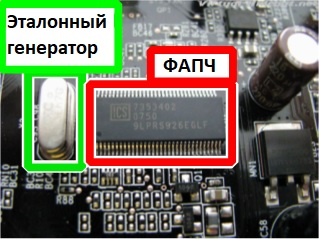
\includegraphics[width=3cm]{images/AppPLL.jpg}
\end{figure}
\end{column}
\hfill
\begin{column}{.5\textwidth}
\begin{figure}
  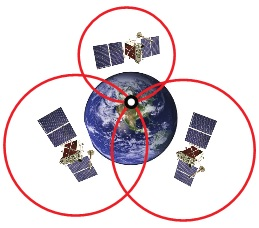
\includegraphics[width=3cm]{images/AppPLL1.jpg}
\end{figure}
\end{column}
\end{columns}

Применение системы ФАПЧ:
\begin{enumerate}
\item Телекоммуникационное обородование
\item Навигационное оборудование (GPS, Глонасс, Галилео)
\item Компьютеры (микропроцессоры)
\end{enumerate}
\end{frame}

%------------------------------------------------

\begin{frame}
\frametitle{Математическая модель ФАПЧ}
\begin{center}
\resizebox{0.9\columnwidth}{!}{%
\begin{tikzpicture}

\node at (0.5,0) [draw, text width=4cm, align=center, rectangle] (a) {Фазовый детектор \par(компаратор)};
\node at (5.2,0) [draw, label=below:{Фильтр}, align=center, rectangle] (loop_filter) {$W(s)$};
\node at (9.6,0) [draw, label={[align=center]below:Генератор,\\управляемый напряжением}] (VCO) {$\omega_{vco}(t) = \omega_{vco}^{free}+K_{vco}\upsilon_f(t)$};

\draw[->] (-3.5,0) -- (a.west) node[midway,above,inner sep=2pt] {sin($\omega_{ref}t$)};
\draw[->] (a.east) -- (loop_filter.west) node[midway,above,inner sep=2pt] {sin($\omega_{e}t$)};
\draw[->] (loop_filter.east) -- (VCO.west) node[midway,above,inner sep=2pt] {$\upsilon_f(t)$};
\draw[->] (VCO.east) -- (14,0) node[midway,above,inner sep=2pt] {cos($\omega_{vco}t$)};
\draw[->] (13.5,0) --  +(0,-2) --  +(-13,-2) --  (a.south);

\end{tikzpicture}
}
\end{center}
Дифференциальные уравнения ФАПЧ
 \begin{equation}\label{system}
 \begin{aligned}
 &\dot{x} = Ax + B(\operatorname{sin}(\theta_e) - \gamma)\text{,}\\[0.3pt]
 &\dot{\theta_e} = -K_{vco}C^T x -K_{vco}D(\operatorname{sin}(\theta_e) - \gamma))\text{,}
 \end{aligned}
\end{equation}
$A$~--- постоянная матрица $n \times n$, $B$ и $C$ постоянные $n$~--- мерные векторы, $D$~--- константа, $x(t)$~--- $n$-мерный вектор состояний системы, $K_{vco}$~--- коэффициент передачи.\vspace{-1mm}
 \begin{equation}\label{gamma}
 \begin{aligned}
\gamma = \frac{\omega_e^{free}}{K_{vco}\left(D-C^T A^{-1}B\right)}\text{,}
 \end{aligned}
\end{equation}
где $\omega^{free}_{e}=\omega_{ref}-\omega_{vco}^{free}$~--- разность частоты опорного сигнала и частоты свободных колебаний ГУН.

\end{frame}

%------------------------------------------------

\begin{frame}
\frametitle{Постановка задачи}
\begin{center}
\resizebox{0.9\columnwidth}{!}{%
\begin{tikzpicture}

\node at (0.5,0) [draw, text width=4cm, align=center, rectangle] (a) {Фазовый детектор \par(компаратор)};
\node at (5.2,0) [draw, label=below:{Фильтр}, align=center, rectangle] (loop_filter) {$W(s)$};
\node at (9.6,0) [draw, label={[align=center]below:Генератор,\\управляемый напряжением}] (VCO) {$\omega_{vco}(t) = \omega_{vco}^{free}+K_{vco}\upsilon_f(t)$};

\draw[->] (-3.5,0) -- (a.west) node[midway,above,inner sep=2pt] {sin($\omega_{ref}t$)};
\draw[->] (a.east) -- (loop_filter.west) node[midway,above,inner sep=2pt] {sin($\omega_{e}t$)};
\draw[->] (loop_filter.east) -- (VCO.west) node[midway,above,inner sep=2pt] {$\upsilon_f(t)$};
\draw[->] (VCO.east) -- (14,0) node[midway,above,inner sep=2pt] {cos($\omega_{vco}t$)};
\draw[->] (13.5,0) --  +(0,-2) --  +(-13,-2) --  (a.south);

\end{tikzpicture}
}
\end{center}
Полоса захвата~--- максимальная разность по модулю частот опорного сигнала и ГУН $|\omega_p|$ такая, что система \eqref{system} глобально асимптотически устойчива для всех $0 \leqslant |\omega_e^{free}|<|\omega_p|$.

Задача: оценить полосы захвата для передаточных функций фильтров:\vspace{-1mm}
\begin{equation*}
 \begin{aligned}
&W(s) = \frac{1}{(1+\tau_{p1}s)(1+\tau_{p2}s)} \text{,} \enskip
W(s) = \frac{(1+\tau_{z1}s)^2}{(1+\tau_{p1}s)^2}\\
&0 < \tau_{pi} < 1 \text{,} \quad 0 < \tau_{zi} < 1  \text{,} \quad i = 1,2 \text{,} \quad \tau_{p1} \neq \tau_{z1}\\
&W(s) = \frac{1+\alpha_1\beta_1s + \alpha_2\beta_2s^2}{1+\alpha_1s + \alpha_2s^2} \text{,} \quad
0 < \beta_1 < \beta_2 < 1 \text{,}\quad 0 < \alpha_1 \text{,} \alpha_2
 \end{aligned}
\end{equation*}
\end{frame}

%------------------------------------------------

\begin{frame}
\frametitle{Теорема}
\vspace{-4mm}
 \begin{equation}\label{system1}
 \begin{aligned}
 &\dot{x} = Ax + B(\operatorname{sin}(\theta_e) - \gamma) \text{,}\\
 &\dot{\theta_e} = -K_{vco}C^T x -K_{vco}D(\operatorname{sin}(\theta_e) - \gamma))
 \end{aligned}
\end{equation}
\vspace{-2.5mm}
Введем обозначение
 \begin{equation}
 \begin{aligned}
\mid\nu\mid = \frac{0,5\pi\gamma}{\gamma \operatorname{arcsin} (\gamma) + \sqrt{1-\gamma^2}}
 \end{aligned}
\end{equation}
\vspace{-3mm}
\begin{theorem}[Леонов~Г.\:А., Райтман~Ф., Смирнова В. Б., 1992 г., Non-Local Methods for
Pendulum-Like Feedback Systems]
Пара $(A, B)$ вполне управляема, все собственные значения матрицы $A$ имеют отрицательные вещественные части и существуют числа $\varepsilon > 0$, $\delta > 0$, $\tau \geqslant 0$, и $\varkappa$, такие что имеют место неравенства:\vspace{-2.5mm}
 \begin{align*}
&\operatorname{Re}\left( \varkappa W(ix)- \varepsilon\left[W(ix)\right]^2-\tau\left[ \overline{W(ix)}+ix \right]\left[W(ix)+ix \right]\right) \geqslant \delta \text{,}\enskip\forall x \in \mathbb{R}\label{first_th_eq}\\
&4\varepsilon\delta > (\varkappa\nu)^2
\end{align*}
Тогда система \eqref{system1} глобально асимптотически устойчива.
\end{theorem}
\end{frame}

%------------------------------------------------

\begin{frame}
\frametitle{Метод решения}
Условия теоремы:\vspace{-2mm}
 \begin{align*}
&\operatorname{Re}\left( \varkappa W(ix)- \varepsilon\left[W(ix)\right]^2-\tau\left[ \overline{W(ix)}+ix \right]\left[W(ix)+ix \right]\right) \geqslant \delta \text{,}\enskip\forall x \in \mathbb{R}\\[-2mm]
&4\varepsilon\delta > (\varkappa\nu)^2
\end{align*}
Для получения оценок полосы захвата необходимо выбрать $\varepsilon, \delta, \varkappa, \tau$, удовлетворяющие первому условию теоремы так, чтобы максимизировать $\nu$. 
Из следующих соотношений получим максимальный $\omega_e^{free}$, при котором система глобально асимптотически устойчива:
 \begin{equation}
 \begin{aligned}
\mid\nu\mid = \frac{0,5\pi\gamma}{\gamma \operatorname{arcsin} (\gamma) + \sqrt{1-\gamma^2}}, \quad \gamma K_{vco}\left(D-C^T A^{-1}B\right)  = \omega_e^{free}
 \end{aligned}
\end{equation}
\end{frame}

%------------------------------------------------

\begin{frame}
\frametitle{Полученные результаты}
\begin{enumerate}
\item Для передаточной функции $W(s) = \frac{1}{(1+\tau_{p1}s)(1+\tau_{p2}s)}$
была найдена оценка полосы захвата
\begin{columns}[onlytextwidth]
\begin{column}{1mm}
\end{column}
\hfill
\begin{column}{.5\textwidth}
\begin{figure}
  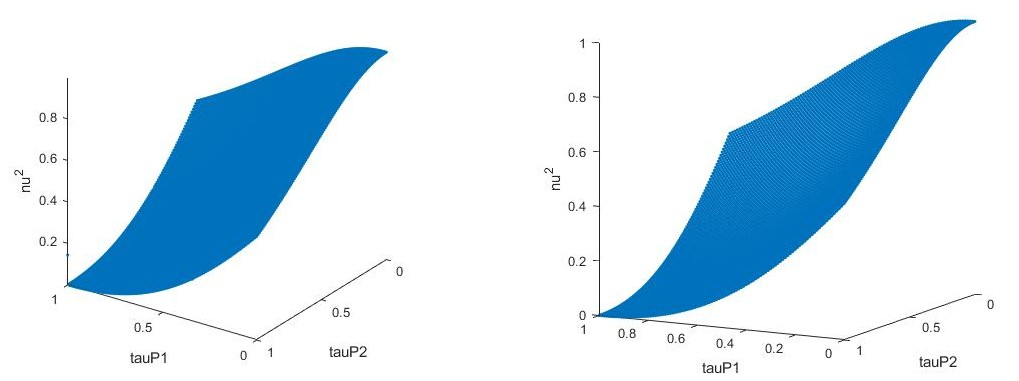
\includegraphics[width=\textwidth]{images/agregated.jpg}
\end{figure}
\end{column}

\begin{column}{.4\textwidth}
\begin{equation*}
 \begin{aligned}
\nu^2 < \frac{(\tau_{p1}\tau_{p2} - 1)^2}{\tau_{p1}^2 + \tau_{p2}^2 + 1}
 \end{aligned}
\end{equation*}
\end{column}
\end{columns}
\item Для передаточной функции $W(s) = \frac{(1+\tau_{z1}s)^2}{(1+\tau_{p1}s)^2}$
была найдена оценка полосы захвата
\begin{columns}[onlytextwidth]
\begin{column}{.3\textwidth}
\begin{figure}
    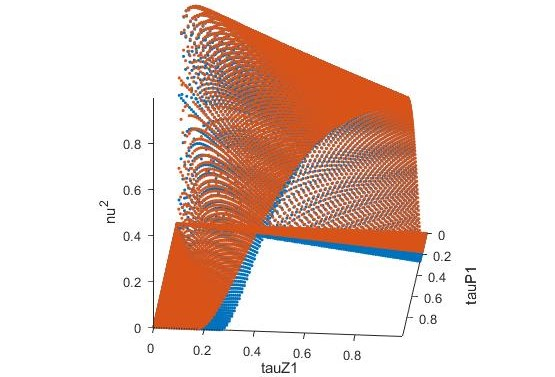
\includegraphics[width=\textwidth]{images/filter2_agregated.jpg}
\end{figure}
\end{column}
\begin{column}{.6\textwidth}
\begin{equation*}
\begin{aligned}
&\nu^2 < \frac{q^2}{z^2}\text{,} \quad 1 \text{,} \quad \frac{4z^2}{1+z^2} \text{,} \quad \frac{4(1-q)(q-z^2)}{1-z^2} \text{,} \\ 
&\frac{z^2-q}{z^2-1} - \left(\frac{z^2-q}{z^2-1}\right)^2
\end{aligned}
\end{equation*}
\end{column}
\end{columns}
\end{enumerate}
\end{frame}

\begin{frame}
\frametitle{Полученные результаты}
\begin{enumerate}
\setcounter{enumi}{2}
\item Для передаточной функции $W(s) = \frac{1+\alpha_1\beta_1s + \alpha_2\beta_2s^2}{1+\alpha_1s + \alpha_2s^2}$ был восстановлен вывод оценки полосы захвата
 \begin{equation*}
\nu^2 < 4\frac{[\alpha_1^2(1-\beta_1) - \alpha_2(1-\beta_2)][\alpha_1^2(1-\beta_1)\beta_1 - \alpha_2(1-\beta_2)]}{[\alpha_1^2(1-\beta_1^2) - 2\alpha_2(1-\beta_2)]^2}
 \end{equation*}
\end{enumerate}
\end{frame}

%------------------------------------------------

\begin{frame}
\Huge{\centerline{Спасибо за внимание}}
\end{frame}

%----------------------------------------------------------------------------------------

\end{document} 